%%
%%  Example paper
%%
%%

%%%%%%%%%%%%%%%%%% Usenix style %%%%%%%%%%%%%%%%%%%%%%%%%%%%%%%%%
\documentclass[10pt,twocolumn,a4paper]{article}
\usepackage{styles/usenix-style}


%%%%%%%%%%%%%%%%%% Document %%%%%%%%%%%%%%%%%%%%%%%%%%%%%%%%%%%%%%%%%%%
% TODO: Change draft to final before submitting final version.
\usepackage[draft]{styles/ka-style}
\usepackage{xspace,ifthen,graphicx,listings}
\setlength{\marginparwidth}{2cm} % to make todonotes fit in twocolumn
\usepackage{todonotes}
\usepackage{glossaries}

\usepackage[
   pdfauthor={Daniel Dietzler},
   pdftitle={Linux Internals},
   pdfsubject={Real-Time Linux},
   pdfkeywords={real-time, rt, linux},
   hidelinks=true
]{hyperref}

\makeglossaries

\usepackage[citestyle=numeric,style=alphabetic,backend=biber]{biblatex}
\addbibresource{seminar-report.bib}

\begin{document}

\newacronym{os}{OSs}{Operating Systems}
\newacronym{rt}{RT}{Real-Time}
\newacronym{rtos}{RTOSs}{Real-Time Operating Systems}
\newacronym{qos}{QoS}{Quality of Service}
\newacronym{pi}{PI}{Priority Inheritance}
\newacronym{rr}{RR}{Round Robin}
\newacronym{fifo}{FIFO}{First In First Out}
\newacronym{gedf}{GEDF}{Global Earliest Deadline First}
\newacronym{rthal}{RTHAL}{Real-Time Hardware Abstraction Layer}
\newacronym{adeos}{ADEOS}{Adaptive Domain Environemnt for Operating Systems}

% Bachelor proseminar: The title simply states your topic.
\title{Real-Time Linux}

% Master's seminar: Ideally, the title already makes clear that this is a report
% on a paper written by other researchers.
\title{%
% document class article doesn't support subtitles, let's hack them
{\normalfont \normalsize Linux Internals Proseminar}\\%
Real-Time Linux \\%
{\normalfont \normalsize \code{PREEMPT\_RT}: Making Linux Real-Time}\\%
{\normalfont \small
Karlsruhe Institute of Technology, ITEC - OS
}%
}

\author{Daniel John Dietzler}

\newcommand{\code}[1]{{\tt \small{#1}}}

\maketitle
%\draftfooter

\begin{abstract}
\end{abstract}

\section{Introduction}\label{sec:introduction}

\acrfull{rtos} are omnipresent in today's connected world.
Ranging from streaming services over networking applications to robotics \cite{buttazzo_hard_1997}, there is an ever-growing need for simpler, yet more feature-rich \acrshort{rtos} \cite{reghenzani_realtime_2019}.
Current solutions are good at being real-time.
However, they generally lack fundamental features such as a fully implemented network stack.
Additionally, \acrshort{rtos} require developers that are specialized in that area.

\section{Real-Time}
\acrfull{rt} requires \emph{temporal determinism}.
That is, a process must terminate within a given time frame for its result to be correct \cite{reghenzani_realtime_2019}.
Additionally, \cite{buttazzo_hard_1997} names four more requirements \acrshort{rt} systems must fulfill:

\begin{itemize}
  \item Efficiency
  \item Robustness (against peak loads)
  \item Fault Tolerance (against hardware failures)
  \item Maintainability
\end{itemize}

\acrshort{rt} can be split up into three levels; \emph{soft}, \emph{firm}, and \emph{hard} \cite{buttazzo_hard_1997}.

\emph{Soft \acrshort{rt}} systems suffer \acrfull{qos} degradation.
That is, a video stream may stutter for instance.
The result however remains valid, although too late.

In \emph{firm \acrshort{rt}} systems, a late result becomes worthless.
It is, as if the result had not been computed in the first place.
A typical example for such systems is the stock exchange \cite{reghenzani_realtime_2019}.
However, a late result does not cause any harm to the system.

Contrary to \emph{firm \acrshort{rt}}, \emph{hard \acrshort{rt}} systems do experience harm if a result is off late.
Missing a deadline here will cause fatal consequences.
Systems where human life is involved are generally considered \emph{hard \acrshort{rt}} \cite{reghenzani_realtime_2019}.
In transportation for instance, a too late reaction can cause the death of people.

\subsection{Real-Time in Linux}
In addition to general \acrshort{rt} properties, a patch of the Linux kernel comes with more challenges \cite{jason_perlow_trenches_2021}.
Required changes are so fundamental that they are very close to the core of the mainline kernel.
As such, the changes need to be as isolated as possible.
They may not block kernel development in any way, and at the same time may be affected by frequent kernel updates \cite{jason_perlow_trenches_2021}.
Additionally, the patches must be as simple as possible.
The mainline Linux kernel is already very complex \footnote{\url{https://github.com/makelinux/linux_kernel_map}}.
Thus, having simple patches helps with maintainability.
Furthermore, related code should be refactored where possible in order to reduce the overall complexity \cite{jason_perlow_trenches_2021}.


\section{History}
The idea of \acrshort{rt} Linux has been around for over two decades \cite{casimiro_how_2000}.
Early on, researchers found interest in making Linux \acrshort{rt} capable.
However, initial efforts were uncoordinated and thus yielded no significant results \cite{jason_perlow_trenches_2021}.
One of the first ideas was to implement a \emph{cokernel}.
While not being the final solution for Linux itself, \emph{cokernel} approaches are used by multiple \acrshort{rtos} today \cite{reghenzani_realtime_2019}.

\subsection{Cokernel}
A \emph{cokernel} describes having a second, separate kernel besides the mainline Linux kernel.
With this, both kernels get threads they can schedule processes on.
Hardware interrupts will be forwarded by a \emph{pico-kernel} \cite{reghenzani_realtime_2019}.
\acrshort{rt} processes will be scheduled on the \acrshort{rt} kernel.
That kernel is optimized for \acrshort{rt} applications and provides \emph{temporal determinism}.
Regular processes will be scheduled on the default, mainline Linux kernel \cite{reghenzani_realtime_2019}.
Having the optimal scheduler for every task by itself is highly efficient.
However, there are issues that must be dealt with.
Cokernel approaches are invasive to the Linux kernel \cite{reghenzani_realtime_2019}.
They require significant modifications and inherently take away control from the mainline kernel.
Additionally, one advantage of having Linux is being able to use the entire ecosystem.
With two kernels communication is expensive, so Linux applications can only be used for non-timely processes \cite{reghenzani_realtime_2019}.
Furthermore, memory swapping between the kernels can lead to page faults and dramatically impact performance \cite{reghenzani_realtime_2019}.
Lastly, with cokernel approaches applications must still be written specifically for the \acrshort{rt} kernel.
This requires specialized developers and multiple versions of the same application \cite{reghenzani_realtime_2019}.

\begin{figure}[hbt]
  \centering
  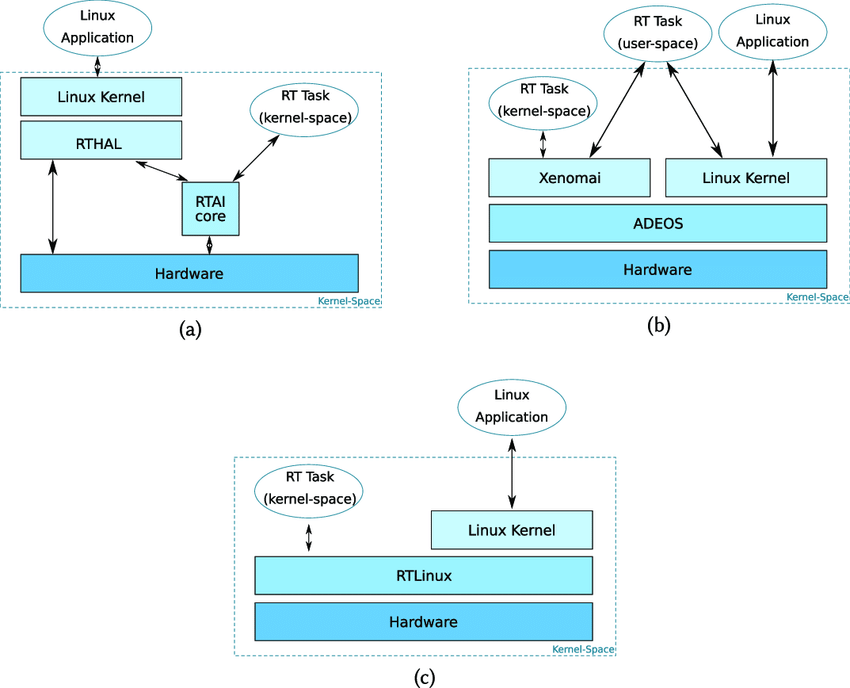
\includegraphics[scale=.26, clip]{assets/cokernel.png}
  \caption{Cokernel approaches. (a) RTAI, (b) Xenomai, (c) RTLinux \cite{reghenzani_realtime_2019} \label{fig:cokernel}}
\end{figure}
Nonetheless, cokernel approaches are broadly represented in today's \acrshort{rtos} landscape.
\emph{RTAI}\footnote{\url{https://www.rtai.org}}, \emph{Xenomai}\footnote{\url{https://xenomai.org}}, and \emph{RTLinux}\footnote{\url{https://en.wikipedia.org/wiki/RTLinux}. Note that this is \emph{not} \acrlong{rt} Linux.} are all popular examples of modern \acrshort{rtos} building on cokernels as can be seen in \autoref{fig:cokernel} \cite{reghenzani_realtime_2019}.
In all cases, the mainline Linux kernel sits on top of a \acrshort{rt} (pico-)kernel.
RTAI uses a pico-kernel called \emph{RTAI core} that schedules \acrshort{rt} kernel space processes.
Then, on top of that there is the \acrfull{rthal} that provides the expected interfaces for the Linux kernel.

Xenomai uses a common pico-kernel called \acrfull{adeos}.
That provides an abstraction layer for both the Xenomai kernel that schedules \acrshort{rt} processes but also the mainline Linux kernel.

Lastly, RTLinux only uses one kernel -- called \emph{RTLinux} -- that provides the hardware abstraction for the Linux kernel as well as \acrshort{rt} scheduling for respective processes.
\newline

\noindent All the uncoordinated efforts towards making Linux \acrshort{rt} led to chaos in 2004 \cite{jason_perlow_trenches_2021}.
In the same year, Ingo Molnar (RedHat) started trying to untangle the chaos.
The goal: \code{PREEMPT\_RT}.
Shortly after, a loose team started to form around Molnar \cite{jason_perlow_trenches_2021}.
Quickly, the team managed to combine the pieces into a working proof of concept \cite{jason_perlow_trenches_2021}.
"[It] was far from a maintainable and production-ready solution", but they "had laid the groundwork and proven that the concept of making the Linux Kernel real-time capable was feasible."\cite{jason_perlow_trenches_2021}
Originally planned for 2018 \cite{lf:history}, \code{PREEMPT\_RT} made it into the LTS kernel in 2024 with kernel version 6.11 \cite{lf:versions}.

\section{Kernel Patch: \code{PREEMPT\_RT}}
In order to make the mainline Linux kernel \acrshort{rt}-capable, many fundamental changes had to be made.
All of those had been grouped in a set of patches called \code{PREEMPT\_RT}.
Firstly, scheduler improvements were necessary in order to improve latencies and timing \cite{mckenney_realtime_2005}.
Potential sections had been identified using new kernel analytics tools, which also discovered new bugs in the mainline kernel \cite{reghenzani_realtime_2019}.
On \acrshort{rtos} context switches happen more frequently due to the nature of \acrshort{rt} applications.
That is, because to guarantee turnaround times, low priority processes need to be preempted if a high priority process comes in \cite{buttazzo_hard_1997}.
This directly leads to secondly, the need to reduce the amount of non-preemptible kernel code \cite{reghenzani_realtime_2019}.
A significant part of the Linux kernel that was non-preemptible were interrupt handlers.

\subsection{Interrupts}
By default, interrupt requests run in the context of the interrupt service routine.
As such, hardware interrupts are disabled for a hard interrupt request, which in turn cause preemption to be disabled \cite{lf:irq}.
With \code{PREEMPT\_RT} a flag allows interrupt handlers to be run in a threaded context instead \cite{reghenzani_realtime_2019, lf:irq}.
This allows to write simple functions that call specialized threads for handling hard interrupt requests\cite{reghenzani_realtime_2019}.
By default, that thread will be scheduled with \code{FIFO} and a high priority of 50 \cite{lf:irq}.

For interrupt handlers that -- under no circumstances -- may run in a threaded context there is an extra flag to disable this behavior per handler \cite{lf:irq}.
Generally one should be careful with this flag though.
It will degrade interrupt performance and scheduling latencies \cite{chyyuu_github_2017, mckenney_realtime_2005}, as well as be prone to deadlocks, making the development of those handlers harder \cite{mckenney_realtime_2005}.
One example for forcing a handler to run in the interrupt context are per-CPU timer interrupts.
With their tight schedules and low level relevance they qualify for being non-preemptible \cite{mckenney_realtime_2005}.
\newline

\noindent In order to further reduce the amount of non-preemptible code, locked, critical sections have been narrowed \cite{mckenney_realtime_2005}.
Additionally, locking mechanisms have been reworked and a new lock got added.

\subsection{Locking}
\subsubsection{General Mechanisms}
Spinlocks are actively waiting for a resource to become available.
They are easy to implement and very fast for shortly waiting process.
This is due to the absence of context switches.
However, they become an increasing problem for longer-waiting processes \cite{lf:sleeping-spinlocks}.

Sleeping mutexes on the other hand are blocking.
When having to wait for a lock they (usually after a short period of spinning) put the thread to sleep.
This comes with two advantages.
First, sleeping mutexes prevent process contention.
That is, multiple processes waiting on a lock and actively hogging resources.
Second, they are also fast.
Instead of wasting CPU cycles waiting for a resource to free, the thread quickly goes to sleep, reducing latencies of other threads.
Most modern implementations of mutexes also have a short spinning period in the beginning, making them performant for shortly waiting processes, too.
\newline

\noindent In the mainline kernel, many locks used to be spinlocks \cite{lf:sleeping-spinlocks}.

\subsubsection{Changes}
With \code{PREEMPT\_RT}, all \code{spinlock\_t} kernel spinlocks have been replaced by \code{rt\_mutex}.

\paragraph{\code{rt\_mutex}} implements \emph{priority inheritance} to avoid the problem of \emph{priority inversion} \cite{rostedt_rtmutex_2017}.
For \code{rt\_mutex}, \acrfull{pi} is implemented by giving each process a \acrshort{pi} \emph{rbtree}, depicting the dependencies of the waiters.
A \acrshort{pi} rbtree of a process stores the top waiter of every lock that is held by that process \cite{rostedt_rtmutex_2017}.
This is called a \acrshort{pi} chain \cite{rostedt_rtmutex_2017}.
Based on this chain, priorities can be changed in order to avoid priority inversion:
A process further right in the chain must always have a priority equal to or higher than processes on the left of it \cite{rostedt_rtmutex_2017}.
\newline

\noindent That change has been done to drastically reduce the amount of spinlocks in the kernel code, making more sections preemptible overall \cite{lf:sleeping-spinlocks}.
However, instead of renaming the type, the team decided to change its implementation depending on whether \code{PREEMPT\_RT} is enabled or not.
This has been done to avoid changing too much kernel code and making pull requests unreviewable \cite{reghenzani_realtime_2019}.
This comes at the expense of non-intuitive kernel code.
If \code{PREEMPT\_RT} is enabled, \code{spinlock\_t} acts as a \code{rt\_mutex}, otherwise it acts as a normal spinlock \cite{mckenney_realtime_2005}.
In case there is need for a genuine spinlock that always behaves as such, \code{raw\_spinlock\_t} can used instead \cite{mckenney_realtime_2005, chyyuu_github_2017}.
\newline

\noindent In order to fulfill \acrshort{rt} requirements, preemption is of utmost importance.
We have already seen how more sections of the kernel code have been made preemptible, and how locking plays a major role in this.
Now, we will focus on the actual preemption.

\subsection{Preemption}
Before the \code{PREEMPT\_RT} patch there have been three preemption modes in the mainline Linux kernel \cite{lf:preemption}.
As described in \cite{lf:preemption} there are
\begin{itemize}
  \item No Forced Preemption (server):
  \item Voluntary Kernel Preemption (desktop):
  \item Preemptible Kernel (low-latency desktop):
\end{itemize}
As the name suggests, \emph{No Forced Preemption} (\code{PREEMPT\_NONE} \cite{mckenney_realtime_2005}) does not have any additional preemption points.
The only scenarios where preemption happens are for system call returns and interrupts.
This is the traditional Linux, with emphasize on throughput.

With \emph{Voluntary Kernel Preemption} (\code{PREEMPT\_VOLUNTARY} \cite{mckenney_realtime_2005}), some explicit preemption points are added to the kernel code.
Specifically \code{might\_sleep()} and \code{might\_sleep\_if()} calls may be preempted \cite{day_re_2007}.
\emph{Voluntary Kernel Preemption} can be found on regular Linux desktops \cite{mckenney_realtime_2005}.

In \emph{Preemptible Kernel} (\code{PREEMPT\_DESKTOP} \cite{mckenney_realtime_2005}) mode, all kernel code that is not running in a critical section becomes preemptible \cite{lf:preemption}.
This reduces the kernel latency ("reactivity") and is thus used in low-latency desktop applications. \cite{mckenney_realtime_2005}.
However, this is not \acrshort{rt} Linux.
\newline

\noindent The \code{PREEMPT\_RT} patch added two new preemption modes to the Linux kernel:
\emph{Preemptible Kernel (basic \acrshort{rt})} and \emph{Fully Preemptible Kernel (\acrshort{rt})} \cite{lf:preemption}.

\emph{Preemptible Kernel (basic \acrshort{rt})} is mainly for debugging purposes.
Its only difference in comparison to \emph{Preemptible Kernel (low-latency desktop)} is that it forces the use of threaded interrupt handlers \cite{lf:preemption}.
Threaded interrupt handlers are preemptible and make up a significant part of the \code{PREEMPT\_RT} patch.

Finally, \emph{Fully Preemptible Kernel} actually marks \acrshort{rt} Linux.
In addition to the aforementioned, most critical sections are preemptible as well, making the Linux kernel broadly preemptible \cite{lf:preemption}.
Furthermore, threaded interrupt handlers are enforced, too.
Substituting spinlocks with \code{rt\_mutex}es as well as breaking up large non-preemptible sections -- as discussed earlier -- lastly give Linux its \acrshort{rt} behavior \cite{lf:preemption}.

\subsection{High Resolution Timers}
Among the most important aspects of a \acrshort{rtos} is a tight scheduler that can very quickly switch between processes \cite{reghenzani_realtime_2019}.
This comes down to two things; (1) preemption and (2) a "good" \acrshort{rt} scheduler.
We have already seen (1), in order to get to (2) we need one more thing though: better timers.
Before \code{PREEMPT\_RT}, system timers could only be set with the precision of the \emph{tick rate} \cite{reghenzani_realtime_2019}.
Now, with the patch, \emph{high resolution timers} were introduced \cite{lf:timers}.
For the first time in Linux, they allow nanosecond-granular timers \cite{reghenzani_realtime_2019}.
This enables better, more reactive scheduling.

\subsection{Scheduler}
Linux has two realtime schedulers; the \emph{(POSIX) realtime scheduler} and the \emph{deadline scheduler} \cite{bristot_de_oliveira_deadline_2018}.
Firstly, the \emph{realtime scheduler} implements \code{SCHED\_FIFO} and \code{SCHED\_RR} \cite{lf:scheduler}.
Both schedule processes based on their fixed priority \cite{lf:scheduler,de_oliveira_timing_2016}.
In \acrfull{fifo} fashion, for processes of the same priority, the process that arrived first will finish running before any other process gets scheduled with \code{SCHED\_FIFO}.
Contrarily, \code{SCHED\_RR} -- using \acrfull{rr} -- will cycle through all processes of the highest priority, giving each process time slices \cite{bristot_de_oliveira_deadline_2018}.

Secondly, the \emph{deadline scheduler} only has one scheduling policy: \code{SCHED\_DEADLINE} \cite{bristot_de_oliveira_deadline_2018}.
That policy implements the \acrfull{gedf} algorithm.
So, instead of making scheduling decisions based on (fixed) priorities, the process with the earliest deadline is considered 'most important' and will be scheduled first \cite{bristot_de_oliveira_deadline_2018}.
Processes scheduled by the \emph{deadline scheduler} can preempt other processes scheduled by the \emph{realtime scheduler} based on \acrshort{fifo} or \acrshort{rr} \cite{lf:scheduler}.

Deadline scheduling is simple for both the user to work with and the scheduler implementation \cite{bristot_de_oliveira_deadline_2018}.
A user does not need to think about priorities.
Especially do they not need to think about other processes, and how those might have impact on their process \cite{bristot_de_oliveira_deadline_2018}.
The user simply has to say when the process needs to have finished, and the scheduler takes care of the rest.

For the implementation of the scheduler, there is no need to analyze any other processes \cite{bristot_de_oliveira_deadline_2018}.
It simply has to always schedule the process with the earliest deadline.
This way, all deadlines are trivially held -- assuming they were possible to meet in the first place \cite{bristot_de_oliveira_deadline_2018}.
This approach also ensures the minimal amount of context switches \cite{bristot_de_oliveira_deadline_2018}.
Only when a process with an earlier deadline than the currently scheduled process comes in does the scheduler need to reschedule and a context switch happens.

However, this approach also comes with downsides.
Inherently, deadline scheduling does not deliver minimal response times \cite{bristot_de_oliveira_deadline_2018}.
Furthermore, "it is possible to face a domino effect" \cite{bristot_de_oliveira_deadline_2018}.
Assuming the process with the earliest deadline has a deadline that's unreachable, because it is too soon.
The scheduler will still schedule that process and "waste" CPU cycles on it, even though it can never finish in time regardless.
This can cause the next process to not meet its deadline as well, even though it could have reached it, if it was scheduled first \cite{bristot_de_oliveira_deadline_2018}.
Thus, such an unmeetable deadline can trickle down to all subsequent processes and cause an entire batch to be off late.


\subsection{Standard Library}
In addition to those fundamental changes to the scheduler, locking, and preemption mechanisms, there were also user-facing libraries that needed updating.
Some essential programs simply had too high latencies for a \acrshort{rt} application \cite{edge_discussion_2022}.
As an example we will be discussing \code{printk}, the kernel equivalent to \code{printf}.

\subsubsection{\code{printk}}
\code{printk} used to have a latency that was "[...] unacceptably high for the real[-]time Linux kernel [...]" \cite{edge_discussion_2022}.
Additionally, a general rework of the library has been long overdue anyways \cite{edge_discussion_2022}.
Lastly, \code{printk} used to use global kernel locks, increasing the latency of the entire system further \cite{gleixner_printk_2024}.
An initial suggestion to make \code{printk} work in \acrshort{rt} Linux boiled down to simply disabling \code{printk} if \code{PREEMPT\_RT} is enabled \cite{mladek_printk_2022}.
Linus Torvalds did not consider this a viable solution and rejected the pull request \cite{torvalds_initial_2022}.

One month later, Thomas Gleixner came up with a new idea on how to improve \code{printk} \cite{gleixner_patch_2022}.
This time around, Linus Torvalds considered the changes acceptable and they got merged in September, 2024 \cite{gleixner_printk_2024}.

\paragraph{Changes.}
Primarily, the global kernel lock has been replaced.
Instead, there are now per-console kernel threads which take care of flushing normal priority messages to the console \cite{gleixner_printk_2024}.
This directly leads to the second addition; priorities.
Every printing process has a priority and needs to check, each time it prints a byte, if it can still print or if there is a process with a higher priority waiting \cite{edge_discussion_2022}.
\emph{panic} messages can do a \emph{hostile takeover} of a console if necessary.
That allows to get as many information to the user before the system or process dies completely \cite{edge_discussion_2022}.
To decide which console to print to, the \code{printk} implementation is now differentiating \emph{safe} and \emph{unsafe} consoles.
For instance, a console becomes \emph{unsafe} if it has experienced a hostile takeover before \cite{kernel_development_community_console}.
In case of a \emph{panic}, the process will always try to print to a save console to increase its chances \cite{gleixner_printk_2024}.
If there is none available, it will try its final flush on an unsafe console and "Hope and pray" \cite{kernel_development_community_console}.


\printglossaries

\printbibliography
%\footnotesize
\end{document}
